\subsection{Implementatie Frontend}
Het laatste deel van de afstudeer applicatie is de \gls{Beheerder} zijn website.
Deze website moet de data van de CMS-API kunnen renderen.
Er is gekozen om een site na te bouwen, de site die hiervoor gekozen is de Snakeware site (Snakeware.com).
Dit is gedaan omdat de developers van de site makkelijk aangesproken kunnen worden voor mogelijke ondersteuning.
Verder is de repository beschikbaar gesteld zodat verschillende stijlingen overgenomen kunnen worden.

\whitespace
Om dit te realiseren is het ontwerp uitgewerkt voor de frontend (zie sectie \ref{sec:FrontendProcessView}).
Het eerste type is de simpelste variant van de frontend onderdelen. 
Het voorbeeld dat gebruikt is rendered een stuk tekst met een titel en optioneel een button.

\whitespace
Dit wordt gedaan door de verschillende \textit{fields} te gebruiken en hiermee de variabelen te vullen.
Deze variabelen worden vervolgens gebruikt in het component om het te renderen op de site.
De implementatie hiervan is te zien in figuur \ref{fig:FrontendImplementatieComponent}.
Verder is er ook te zien dat de \qw{Link} field gebruikt wordt om  een redirect uit te voeren zodra er opgeklikt wordt.

\whitespace
\begin{graphic}
    \captionsetup{type=figure}
    \caption{Implemenatie van Vue component}
    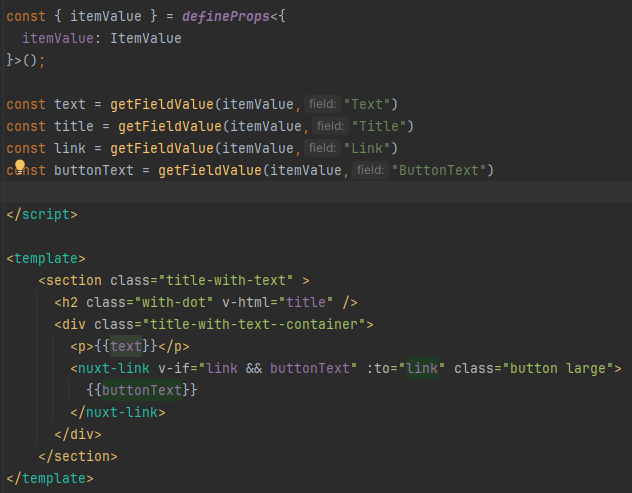
\includegraphics[scale=0.8]{ImplementationOfComponentVue.png}
    \label{fig:FrontendImplementatieComhoe dit uit in de datastructuuronent}
\end{graphic}

\whitespace
Het tweede type component is een Container component die te zien is in figuur \ref{fig:FrontendContainerImplementatie}.
Dit component rendered alle \qw{implementatie componenten} dit wordt gedaan door gebruik te maken van het component \qw{component}.
Het \qw{component} component wordt ook wel v-component genoemd om de verwarringen te voorkomen.
Dit v-component kan gerenderd worden als elk component dat je mee geeft.
Hierdoor is het makkelijk om op run time te bepalen welk component gerenderd moet worden.
Verder wordt het Container zelf ook gebruikt als het item geen fields heeft.
Hierdoor kan de content recursief gerenderd worden.

\newpage

\whitespace
\begin{graphic}
    \captionsetup{type=figure}
    \caption{Implementatie container component}
    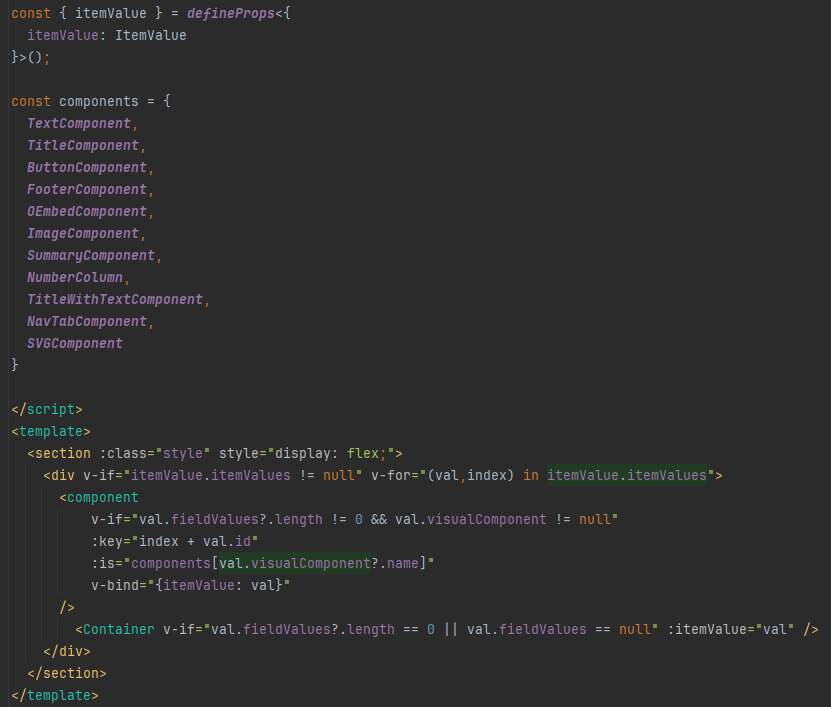
\includegraphics[scale=0.5]{ImplementatieContainersVue.png}
    \label{fig:FrontendContainerImplementatie}
\end{graphic}

\whitespace
Door het gebruik te maken van deze 2 type componenten is het mogelijk om de snakeware site te renderen.
De volledige rendering van de site is te zien in figuur \ref{fig:Frontend}.

\whitespace
\begin{graphic}
    \captionsetup{type=figure}
    \caption{Frontend}
    
\includegraphics[scale=0.3]{Placeholder.jpg}
    \label{fig:Frontend}
\end{graphic}

\todo[inline]{Wil ik als laatste doen}
